\documentclass[1p]{elsarticle_modified}
%\bibliographystyle{elsarticle-num}

%\usepackage[colorlinks]{hyperref}
%\usepackage{abbrmath_seonhwa} %\Abb, \Ascr, \Acal ,\Abf, \Afrak
\usepackage{amsfonts}
\usepackage{amssymb}
\usepackage{amsmath}
\usepackage{amsthm}
\usepackage{scalefnt}
\usepackage{amsbsy}
\usepackage{kotex}
\usepackage{caption}
\usepackage{subfig}
\usepackage{color}
\usepackage{graphicx}
\usepackage{xcolor} %% white, black, red, green, blue, cyan, magenta, yellow
\usepackage{float}
\usepackage{setspace}
\usepackage{hyperref}

\usepackage{tikz}
\usetikzlibrary{arrows}

\usepackage{multirow}
\usepackage{array} % fixed length table
\usepackage{hhline}

%%%%%%%%%%%%%%%%%%%%%
\makeatletter
\renewcommand*\env@matrix[1][\arraystretch]{%
	\edef\arraystretch{#1}%
	\hskip -\arraycolsep
	\let\@ifnextchar\new@ifnextchar
	\array{*\c@MaxMatrixCols c}}
\makeatother %https://tex.stackexchange.com/questions/14071/how-can-i-increase-the-line-spacing-in-a-matrix
%%%%%%%%%%%%%%%

\usepackage[normalem]{ulem}

\newcommand{\msout}[1]{\ifmmode\text{\sout{\ensuremath{#1}}}\else\sout{#1}\fi}
%SOURCE: \msout is \stkout macro in https://tex.stackexchange.com/questions/20609/strikeout-in-math-mode

\newcommand{\cancel}[1]{
	\ifmmode
	{\color{red}\msout{#1}}
	\else
	{\color{red}\sout{#1}}
	\fi
}

\newcommand{\add}[1]{
	{\color{blue}\uwave{#1}}
}

\newcommand{\replace}[2]{
	\ifmmode
	{\color{red}\msout{#1}}{\color{blue}\uwave{#2}}
	\else
	{\color{red}\sout{#1}}{\color{blue}\uwave{#2}}
	\fi
}

\newcommand{\Sol}{\mathcal{S}} %segment
\newcommand{\D}{D} %diagram
\newcommand{\A}{\mathcal{A}} %arc


%%%%%%%%%%%%%%%%%%%%%%%%%%%%%5 test

\def\sl{\operatorname{\textup{SL}}(2,\Cbb)}
\def\psl{\operatorname{\textup{PSL}}(2,\Cbb)}
\def\quan{\mkern 1mu \triangleright \mkern 1mu}

\theoremstyle{definition}
\newtheorem{thm}{Theorem}[section]
\newtheorem{prop}[thm]{Proposition}
\newtheorem{lem}[thm]{Lemma}
\newtheorem{ques}[thm]{Question}
\newtheorem{cor}[thm]{Corollary}
\newtheorem{defn}[thm]{Definition}
\newtheorem{exam}[thm]{Example}
\newtheorem{rmk}[thm]{Remark}
\newtheorem{alg}[thm]{Algorithm}

\newcommand{\I}{\sqrt{-1}}
\begin{document}

%\begin{frontmatter}
%
%\title{Boundary parabolic representations of knots up to 8 crossings}
%
%%% Group authors per affiliation:
%\author{Yunhi Cho} 
%\address{Department of Mathematics, University of Seoul, Seoul, Korea}
%\ead{yhcho@uos.ac.kr}
%
%
%\author{Seonhwa Kim} %\fnref{s_kim}}
%\address{Center for Geometry and Physics, Institute for Basic Science, Pohang, 37673, Korea}
%\ead{ryeona17@ibs.re.kr}
%
%\author{Hyuk Kim}
%\address{Department of Mathematical Sciences, Seoul National University, Seoul 08826, Korea}
%\ead{hyukkim@snu.ac.kr}
%
%\author{Seokbeom Yoon}
%\address{Department of Mathematical Sciences, Seoul National University, Seoul, 08826,  Korea}
%\ead{sbyoon15@snu.ac.kr}
%
%\begin{abstract}
%We find all boundary parabolic representation of knots up to 8 crossings.
%
%\end{abstract}
%\begin{keyword}
%    \MSC[2010] 57M25 
%\end{keyword}
%
%\end{frontmatter}

%\linenumbers
%\tableofcontents
%
\newcommand\colored[1]{\textcolor{white}{\rule[-0.35ex]{0.8em}{1.4ex}}\kern-0.8em\color{red} #1}%
%\newcommand\colored[1]{\textcolor{white}{ #1}\kern-2.17ex	\textcolor{white}{ #1}\kern-1.81ex	\textcolor{white}{ #1}\kern-2.15ex\color{red}#1	}

{\Large $\underline{12n_{0162}~(K12n_{0162})}$}

\setlength{\tabcolsep}{10pt}
\renewcommand{\arraystretch}{1.6}
\vspace{1cm}\begin{tabular}{m{100pt}>{\centering\arraybackslash}m{274pt}}
\multirow{5}{120pt}{
	\centering
	\includegraphics[width=112pt]{../../../GIT/diagram.site/Diagrams/png/2251_12n_0162.png}\\
\ \ \ A knot diagram\footnotemark}&
\allowdisplaybreaks
\textbf{Linearized knot diagam} \\
\cline{2-2}
 &
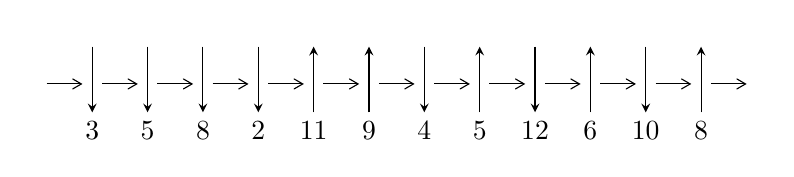
\begin{tikzpicture}[x=20pt, y=17pt]
	% nodes
	\node (C0) at (0, 0) {};
	\node (C1) at (1, 0) {};
	\node (C1U) at (1, +1) {};
	\node (C1D) at (1, -1) {3};

	\node (C2) at (2, 0) {};
	\node (C2U) at (2, +1) {};
	\node (C2D) at (2, -1) {5};

	\node (C3) at (3, 0) {};
	\node (C3U) at (3, +1) {};
	\node (C3D) at (3, -1) {8};

	\node (C4) at (4, 0) {};
	\node (C4U) at (4, +1) {};
	\node (C4D) at (4, -1) {2};

	\node (C5) at (5, 0) {};
	\node (C5U) at (5, +1) {};
	\node (C5D) at (5, -1) {11};

	\node (C6) at (6, 0) {};
	\node (C6U) at (6, +1) {};
	\node (C6D) at (6, -1) {9};

	\node (C7) at (7, 0) {};
	\node (C7U) at (7, +1) {};
	\node (C7D) at (7, -1) {4};

	\node (C8) at (8, 0) {};
	\node (C8U) at (8, +1) {};
	\node (C8D) at (8, -1) {5};

	\node (C9) at (9, 0) {};
	\node (C9U) at (9, +1) {};
	\node (C9D) at (9, -1) {12};

	\node (C10) at (10, 0) {};
	\node (C10U) at (10, +1) {};
	\node (C10D) at (10, -1) {6};

	\node (C11) at (11, 0) {};
	\node (C11U) at (11, +1) {};
	\node (C11D) at (11, -1) {10};

	\node (C12) at (12, 0) {};
	\node (C12U) at (12, +1) {};
	\node (C12D) at (12, -1) {8};
	\node (C13) at (13, 0) {};

	% arrows
	\draw[->,>={angle 60}]
	(C0) edge (C1) (C1) edge (C2) (C2) edge (C3) (C3) edge (C4) (C4) edge (C5) (C5) edge (C6) (C6) edge (C7) (C7) edge (C8) (C8) edge (C9) (C9) edge (C10) (C10) edge (C11) (C11) edge (C12) (C12) edge (C13) ;	\draw[->,>=stealth]
	(C1U) edge (C1D) (C2U) edge (C2D) (C3U) edge (C3D) (C4U) edge (C4D) (C5D) edge (C5U) (C6D) edge (C6U) (C7U) edge (C7D) (C8D) edge (C8U) (C9U) edge (C9D) (C10D) edge (C10U) (C11U) edge (C11D) (C12D) edge (C12U) ;
	\end{tikzpicture} \\
\hhline{~~} \\& 
\textbf{Solving Sequence} \\ \cline{2-2} 
 &
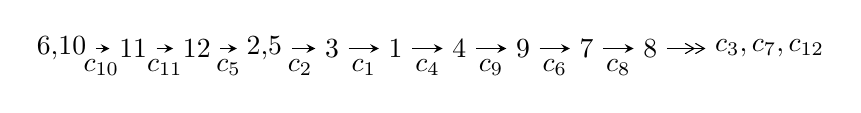
\begin{tikzpicture}[x=23pt, y=7pt]
	% node
	\node (A0) at (-1/8, 0) {6,10};
	\node (A1) at (1, 0) {11};
	\node (A2) at (2, 0) {12};
	\node (A3) at (49/16, 0) {2,5};
	\node (A4) at (33/8, 0) {3};
	\node (A5) at (41/8, 0) {1};
	\node (A6) at (49/8, 0) {4};
	\node (A7) at (57/8, 0) {9};
	\node (A8) at (65/8, 0) {7};
	\node (A9) at (73/8, 0) {8};
	\node (C1) at (1/2, -1) {$c_{10}$};
	\node (C2) at (3/2, -1) {$c_{11}$};
	\node (C3) at (5/2, -1) {$c_{5}$};
	\node (C4) at (29/8, -1) {$c_{2}$};
	\node (C5) at (37/8, -1) {$c_{1}$};
	\node (C6) at (45/8, -1) {$c_{4}$};
	\node (C7) at (53/8, -1) {$c_{9}$};
	\node (C8) at (61/8, -1) {$c_{6}$};
	\node (C9) at (69/8, -1) {$c_{8}$};
	\node (A10) at (11, 0) {$c_{3},c_{7},c_{12}$};

	% edge
	\draw[->,>=stealth]	
	(A0) edge (A1) (A1) edge (A2) (A2) edge (A3) (A3) edge (A4) (A4) edge (A5) (A5) edge (A6) (A6) edge (A7) (A7) edge (A8) (A8) edge (A9) ;
	\draw[->>,>={angle 60}]	
	(A9) edge (A10);
\end{tikzpicture} \\ 

\end{tabular} \\

\footnotetext{
The image of knot diagram is generated by the software ``\textbf{Draw programme}" developed by Andrew Bartholomew(\url{http://www.layer8.co.uk/maths/draw/index.htm\#Running-draw}), where we modified some parts for our purpose(\url{https://github.com/CATsTAILs/LinksPainter}).
}\phantom \\ \newline 
\centering \textbf{Ideals for irreducible components\footnotemark of $X_{\text{par}}$} 
 
\begin{align*}
I^u_{1}&=\langle 
2 u^{38}-4 u^{37}+\cdots+b-2,\;-2 u^{38}+2 u^{37}+\cdots+a+3,\;u^{39}-2 u^{38}+\cdots+2 u+1\rangle \\
I^u_{2}&=\langle 
- u^7- u^5- u^3+u^2+b,\;- u^6- u^4-2 u^2+a-1,\;u^9+u^8+2 u^7+u^6+3 u^5+u^4+2 u^3+u-1\rangle \\
\\
\end{align*}
\raggedright * 2 irreducible components of $\dim_{\mathbb{C}}=0$, with total 48 representations.\\
\footnotetext{All coefficients of polynomials are rational numbers. But the coefficients are sometimes approximated in decimal forms when there is not enough margin.}
\newpage
\renewcommand{\arraystretch}{1}
\centering \section*{I. $I^u_{1}= \langle 2 u^{38}-4 u^{37}+\cdots+b-2,\;-2 u^{38}+2 u^{37}+\cdots+a+3,\;u^{39}-2 u^{38}+\cdots+2 u+1 \rangle$}
\flushleft \textbf{(i) Arc colorings}\\
\begin{tabular}{m{7pt} m{180pt} m{7pt} m{180pt} }
\flushright $a_{6}=$&$\begin{pmatrix}0\\u\end{pmatrix}$ \\
\flushright $a_{10}=$&$\begin{pmatrix}1\\0\end{pmatrix}$ \\
\flushright $a_{11}=$&$\begin{pmatrix}1\\- u^2\end{pmatrix}$ \\
\flushright $a_{12}=$&$\begin{pmatrix}u^2+1\\- u^2\end{pmatrix}$ \\
\flushright $a_{2}=$&$\begin{pmatrix}2 u^{38}-2 u^{37}+\cdots+3 u-3\\-2 u^{38}+4 u^{37}+\cdots+6 u+2\end{pmatrix}$ \\
\flushright $a_{5}=$&$\begin{pmatrix}- u\\u^3+u\end{pmatrix}$ \\
\flushright $a_{3}=$&$\begin{pmatrix}3 u^{38}-3 u^{37}+\cdots+3 u-3\\-3 u^{38}+6 u^{37}+\cdots+9 u+3\end{pmatrix}$ \\
\flushright $a_{1}=$&$\begin{pmatrix}- u^{20}-3 u^{18}-7 u^{16}-10 u^{14}-10 u^{12}-7 u^{10}- u^8+2 u^6+3 u^4+u^2-1\\u^{22}+4 u^{20}+\cdots+2 u^4+u^2\end{pmatrix}$ \\
\flushright $a_{4}=$&$\begin{pmatrix}u^{38}- u^{37}+\cdots+3 u-2\\- u^{38}+2 u^{37}+\cdots+4 u+1\end{pmatrix}$ \\
\flushright $a_{9}=$&$\begin{pmatrix}u^4+u^2+1\\- u^4\end{pmatrix}$ \\
\flushright $a_{7}=$&$\begin{pmatrix}u^9+2 u^7+3 u^5+2 u^3+u\\- u^9- u^7- u^5+u\end{pmatrix}$ \\
\flushright $a_{8}=$&$\begin{pmatrix}- u^8- u^6- u^4+1\\u^{10}+2 u^8+3 u^6+2 u^4+u^2\end{pmatrix}$\\&\end{tabular}
\flushleft \textbf{(ii) Obstruction class $= -1$}\\~\\
\flushleft \textbf{(iii) Cusp Shapes $= -4 u^{38}+6 u^{37}-28 u^{36}+32 u^{35}-120 u^{34}+122 u^{33}-369 u^{32}+323 u^{31}-893 u^{30}+680 u^{29}-1762 u^{28}+1139 u^{27}-2917 u^{26}+1542 u^{25}-4078 u^{24}+1638 u^{23}-4860 u^{22}+1250 u^{21}-4902 u^{20}+407 u^{19}-4141 u^{18}-578 u^{17}-2860 u^{16}-1302 u^{15}-1518 u^{14}-1484 u^{13}-540 u^{12}-1166 u^{11}-62 u^{10}-622 u^9+52 u^8-188 u^7+8 u^6+28 u^5-32 u^4+47 u^3-17 u^2+8 u-6$}\\~\\
\newpage\renewcommand{\arraystretch}{1}
\flushleft \textbf{(iv) u-Polynomials at the component}\newline \\
\begin{tabular}{m{50pt}|m{274pt}}
Crossings & \hspace{64pt}u-Polynomials at each crossing \\
\hline $$\begin{aligned}c_{1}\end{aligned}$$&$\begin{aligned}
&u^{39}+4 u^{38}+\cdots+6 u+1
\end{aligned}$\\
\hline $$\begin{aligned}c_{2},c_{4}\end{aligned}$$&$\begin{aligned}
&u^{39}-10 u^{38}+\cdots-10 u+1
\end{aligned}$\\
\hline $$\begin{aligned}c_{3},c_{7}\end{aligned}$$&$\begin{aligned}
&u^{39}+u^{38}+\cdots+1024 u+512
\end{aligned}$\\
\hline $$\begin{aligned}c_{5},c_{10}\end{aligned}$$&$\begin{aligned}
&u^{39}-2 u^{38}+\cdots+2 u+1
\end{aligned}$\\
\hline $$\begin{aligned}c_{6}\end{aligned}$$&$\begin{aligned}
&u^{39}+10 u^{38}+\cdots+1722 u+193
\end{aligned}$\\
\hline $$\begin{aligned}c_{8}\end{aligned}$$&$\begin{aligned}
&u^{39}-2 u^{38}+\cdots+2 u+1
\end{aligned}$\\
\hline $$\begin{aligned}c_{9},c_{11}\end{aligned}$$&$\begin{aligned}
&u^{39}+12 u^{38}+\cdots+18 u-1
\end{aligned}$\\
\hline $$\begin{aligned}c_{12}\end{aligned}$$&$\begin{aligned}
&u^{39}+8 u^{38}+\cdots+1136340 u-591991
\end{aligned}$\\
\hline
\end{tabular}\\~\\
\newpage\renewcommand{\arraystretch}{1}
\flushleft \textbf{(v) Riley Polynomials at the component}\newline \\
\begin{tabular}{m{50pt}|m{274pt}}
Crossings & \hspace{64pt}Riley Polynomials at each crossing \\
\hline $$\begin{aligned}c_{1}\end{aligned}$$&$\begin{aligned}
&y^{39}+72 y^{38}+\cdots+42 y-1
\end{aligned}$\\
\hline $$\begin{aligned}c_{2},c_{4}\end{aligned}$$&$\begin{aligned}
&y^{39}-4 y^{38}+\cdots+6 y-1
\end{aligned}$\\
\hline $$\begin{aligned}c_{3},c_{7}\end{aligned}$$&$\begin{aligned}
&y^{39}+57 y^{38}+\cdots-3145728 y-262144
\end{aligned}$\\
\hline $$\begin{aligned}c_{5},c_{10}\end{aligned}$$&$\begin{aligned}
&y^{39}+12 y^{38}+\cdots+18 y-1
\end{aligned}$\\
\hline $$\begin{aligned}c_{6}\end{aligned}$$&$\begin{aligned}
&y^{39}-20 y^{38}+\cdots+882042 y-37249
\end{aligned}$\\
\hline $$\begin{aligned}c_{8}\end{aligned}$$&$\begin{aligned}
&y^{39}-52 y^{38}+\cdots+18 y-1
\end{aligned}$\\
\hline $$\begin{aligned}c_{9},c_{11}\end{aligned}$$&$\begin{aligned}
&y^{39}+32 y^{38}+\cdots+438 y-1
\end{aligned}$\\
\hline $$\begin{aligned}c_{12}\end{aligned}$$&$\begin{aligned}
&y^{39}-112 y^{38}+\cdots+32115490504994 y-350453344081
\end{aligned}$\\
\hline
\end{tabular}\\~\\
\newpage\flushleft \textbf{(vi) Complex Volumes and Cusp Shapes}
$$\begin{array}{c|c|c}  
\text{Solutions to }I^u_{1}& \I (\text{vol} + \sqrt{-1}CS) & \text{Cusp shape}\\
 \hline 
\begin{aligned}
u &= \phantom{-}0.120246 + 1.009060 I \\
a &= \phantom{-}0.245784 - 1.091900 I \\
b &= \phantom{-}0.063842 + 0.428041 I\end{aligned}
 & -2.16299 + 2.79564 I & -3.22234 - 5.02358 I \\ \hline\begin{aligned}
u &= \phantom{-}0.120246 - 1.009060 I \\
a &= \phantom{-}0.245784 + 1.091900 I \\
b &= \phantom{-}0.063842 - 0.428041 I\end{aligned}
 & -2.16299 - 2.79564 I & -3.22234 + 5.02358 I \\ \hline\begin{aligned}
u &= -0.784016 + 0.696729 I \\
a &= \phantom{-}1.54879 + 0.28318 I \\
b &= -1.30776 + 1.31337 I\end{aligned}
 & \phantom{-}3.90920 + 2.54093 I & \phantom{-}3.58364 - 2.83796 I \\ \hline\begin{aligned}
u &= -0.784016 - 0.696729 I \\
a &= \phantom{-}1.54879 - 0.28318 I \\
b &= -1.30776 - 1.31337 I\end{aligned}
 & \phantom{-}3.90920 - 2.54093 I & \phantom{-}3.58364 + 2.83796 I \\ \hline\begin{aligned}
u &= \phantom{-}0.596432 + 0.887614 I \\
a &= -0.515948 - 0.665357 I \\
b &= -0.671166 + 1.160530 I\end{aligned}
 & \phantom{-}0.19918 + 2.33431 I & \phantom{-}0.66043 - 2.69942 I \\ \hline\begin{aligned}
u &= \phantom{-}0.596432 - 0.887614 I \\
a &= -0.515948 + 0.665357 I \\
b &= -0.671166 - 1.160530 I\end{aligned}
 & \phantom{-}0.19918 - 2.33431 I & \phantom{-}0.66043 + 2.69942 I \\ \hline\begin{aligned}
u &= -0.293261 + 1.042380 I \\
a &= \phantom{-}0.412665 + 0.456169 I \\
b &= \phantom{-}0.948855 + 0.872815 I\end{aligned}
 & \phantom{-}7.61588 + 0.58808 I & -2.37285 + 1.24200 I \\ \hline\begin{aligned}
u &= -0.293261 - 1.042380 I \\
a &= \phantom{-}0.412665 - 0.456169 I \\
b &= \phantom{-}0.948855 - 0.872815 I\end{aligned}
 & \phantom{-}7.61588 - 0.58808 I & -2.37285 - 1.24200 I \\ \hline\begin{aligned}
u &= -0.248492 + 1.061350 I \\
a &= -1.15816 - 0.97210 I \\
b &= -0.264108 + 0.521722 I\end{aligned}
 & \phantom{-}7.32167 - 7.23317 I & -2.97850 + 5.46930 I \\ \hline\begin{aligned}
u &= -0.248492 - 1.061350 I \\
a &= -1.15816 + 0.97210 I \\
b &= -0.264108 - 0.521722 I\end{aligned}
 & \phantom{-}7.32167 + 7.23317 I & -2.97850 - 5.46930 I\\
 \hline 
 \end{array}$$\newpage$$\begin{array}{c|c|c}  
\text{Solutions to }I^u_{1}& \I (\text{vol} + \sqrt{-1}CS) & \text{Cusp shape}\\
 \hline 
\begin{aligned}
u &= \phantom{-}0.727925 + 0.815935 I \\
a &= \phantom{-}1.03158 - 1.88331 I \\
b &= -2.28549 + 0.08879 I\end{aligned}
 & \phantom{-}1.36861 + 0.67210 I & -0.227831 - 0.290291 I \\ \hline\begin{aligned}
u &= \phantom{-}0.727925 - 0.815935 I \\
a &= \phantom{-}1.03158 + 1.88331 I \\
b &= -2.28549 - 0.08879 I\end{aligned}
 & \phantom{-}1.36861 - 0.67210 I & -0.227831 + 0.290291 I \\ \hline\begin{aligned}
u &= \phantom{-}0.219912 + 0.863651 I \\
a &= -0.840864 - 0.340640 I \\
b &= -0.408735 + 0.084317 I\end{aligned}
 & -0.71566 + 1.83000 I & -2.05496 - 5.14676 I \\ \hline\begin{aligned}
u &= \phantom{-}0.219912 - 0.863651 I \\
a &= -0.840864 + 0.340640 I \\
b &= -0.408735 - 0.084317 I\end{aligned}
 & -0.71566 - 1.83000 I & -2.05496 + 5.14676 I \\ \hline\begin{aligned}
u &= -0.699877 + 0.873292 I \\
a &= -0.469502 + 0.267136 I \\
b &= -0.70229 - 1.61147 I\end{aligned}
 & -0.05262 - 2.68764 I & \phantom{-}1.74155 + 3.66223 I \\ \hline\begin{aligned}
u &= -0.699877 - 0.873292 I \\
a &= -0.469502 - 0.267136 I \\
b &= -0.70229 + 1.61147 I\end{aligned}
 & -0.05262 + 2.68764 I & \phantom{-}1.74155 - 3.66223 I \\ \hline\begin{aligned}
u &= -0.801951 + 0.791302 I \\
a &= -1.14040 - 0.96544 I \\
b &= \phantom{-}1.86997 + 0.11290 I\end{aligned}
 & \phantom{-}5.59974 - 0.03074 I & \phantom{-}4.36542 + 0.32402 I \\ \hline\begin{aligned}
u &= -0.801951 - 0.791302 I \\
a &= -1.14040 + 0.96544 I \\
b &= \phantom{-}1.86997 - 0.11290 I\end{aligned}
 & \phantom{-}5.59974 + 0.03074 I & \phantom{-}4.36542 - 0.32402 I \\ \hline\begin{aligned}
u &= \phantom{-}0.864121 + 0.732996 I \\
a &= -1.98825 + 1.82338 I \\
b &= \phantom{-}3.31808 + 0.25253 I\end{aligned}
 & \phantom{-}14.7085 - 6.7067 I & \phantom{-}2.84933 + 2.28339 I \\ \hline\begin{aligned}
u &= \phantom{-}0.864121 - 0.732996 I \\
a &= -1.98825 - 1.82338 I \\
b &= \phantom{-}3.31808 - 0.25253 I\end{aligned}
 & \phantom{-}14.7085 + 6.7067 I & \phantom{-}2.84933 - 2.28339 I\\
 \hline 
 \end{array}$$\newpage$$\begin{array}{c|c|c}  
\text{Solutions to }I^u_{1}& \I (\text{vol} + \sqrt{-1}CS) & \text{Cusp shape}\\
 \hline 
\begin{aligned}
u &= -0.060322 + 0.863529 I \\
a &= \phantom{-}1.31866 + 0.55049 I \\
b &= -0.236777 - 1.257920 I\end{aligned}
 & -3.43952 - 0.92375 I & -7.85826 - 1.02249 I \\ \hline\begin{aligned}
u &= -0.060322 - 0.863529 I \\
a &= \phantom{-}1.31866 - 0.55049 I \\
b &= -0.236777 + 1.257920 I\end{aligned}
 & -3.43952 + 0.92375 I & -7.85826 + 1.02249 I \\ \hline\begin{aligned}
u &= \phantom{-}0.863742 + 0.759791 I \\
a &= \phantom{-}1.91967 + 0.29557 I \\
b &= -1.83974 - 1.49581 I\end{aligned}
 & \phantom{-}15.2033 + 1.5546 I & \phantom{-}3.37626 - 1.94136 I \\ \hline\begin{aligned}
u &= \phantom{-}0.863742 - 0.759791 I \\
a &= \phantom{-}1.91967 - 0.29557 I \\
b &= -1.83974 + 1.49581 I\end{aligned}
 & \phantom{-}15.2033 - 1.5546 I & \phantom{-}3.37626 + 1.94136 I \\ \hline\begin{aligned}
u &= \phantom{-}0.718483 + 0.920822 I \\
a &= -1.98095 + 0.84172 I \\
b &= \phantom{-}2.64227 + 1.17341 I\end{aligned}
 & \phantom{-}1.04684 + 4.85277 I & -1.08190 - 5.10627 I \\ \hline\begin{aligned}
u &= \phantom{-}0.718483 - 0.920822 I \\
a &= -1.98095 - 0.84172 I \\
b &= \phantom{-}2.64227 - 1.17341 I\end{aligned}
 & \phantom{-}1.04684 - 4.85277 I & -1.08190 + 5.10627 I \\ \hline\begin{aligned}
u &= -0.756351 + 0.955946 I \\
a &= \phantom{-}1.29073 + 0.97706 I \\
b &= -1.70884 + 0.75010 I\end{aligned}
 & \phantom{-}5.09426 - 5.82741 I & \phantom{-}3.18362 + 5.23319 I \\ \hline\begin{aligned}
u &= -0.756351 - 0.955946 I \\
a &= \phantom{-}1.29073 - 0.97706 I \\
b &= -1.70884 - 0.75010 I\end{aligned}
 & \phantom{-}5.09426 + 5.82741 I & \phantom{-}3.18362 - 5.23319 I \\ \hline\begin{aligned}
u &= -0.711811 + 0.997242 I \\
a &= -0.37938 - 1.46724 I \\
b &= \phantom{-}2.21221 + 0.85051 I\end{aligned}
 & \phantom{-}3.00218 - 8.19358 I & \phantom{-}1.84671 + 8.19526 I \\ \hline\begin{aligned}
u &= -0.711811 - 0.997242 I \\
a &= -0.37938 + 1.46724 I \\
b &= \phantom{-}2.21221 - 0.85051 I\end{aligned}
 & \phantom{-}3.00218 + 8.19358 I & \phantom{-}1.84671 - 8.19526 I\\
 \hline 
 \end{array}$$\newpage$$\begin{array}{c|c|c}  
\text{Solutions to }I^u_{1}& \I (\text{vol} + \sqrt{-1}CS) & \text{Cusp shape}\\
 \hline 
\begin{aligned}
u &= \phantom{-}0.777121 + 1.000210 I \\
a &= -0.10510 + 1.98160 I \\
b &= \phantom{-}1.90838 - 0.99134 I\end{aligned}
 & \phantom{-}14.4580 + 4.5482 I & \phantom{-}2.23048 - 2.92809 I \\ \hline\begin{aligned}
u &= \phantom{-}0.777121 - 1.000210 I \\
a &= -0.10510 - 1.98160 I \\
b &= \phantom{-}1.90838 + 0.99134 I\end{aligned}
 & \phantom{-}14.4580 - 4.5482 I & \phantom{-}2.23048 + 2.92809 I \\ \hline\begin{aligned}
u &= \phantom{-}0.764056 + 1.013960 I \\
a &= \phantom{-}2.01030 - 1.76059 I \\
b &= -3.73540 - 0.89810 I\end{aligned}
 & \phantom{-}13.8390 + 12.7651 I & \phantom{-}1.42561 - 7.10495 I \\ \hline\begin{aligned}
u &= \phantom{-}0.764056 - 1.013960 I \\
a &= \phantom{-}2.01030 + 1.76059 I \\
b &= -3.73540 + 0.89810 I\end{aligned}
 & \phantom{-}13.8390 - 12.7651 I & \phantom{-}1.42561 + 7.10495 I \\ \hline\begin{aligned}
u &= -0.727545 + 0.029883 I \\
a &= \phantom{-}0.918981 + 0.363391 I \\
b &= -0.008973 + 1.054810 I\end{aligned}
 & \phantom{-}10.90740 - 4.01643 I & \phantom{-}3.18279 + 2.27518 I \\ \hline\begin{aligned}
u &= -0.727545 - 0.029883 I \\
a &= \phantom{-}0.918981 - 0.363391 I \\
b &= -0.008973 - 1.054810 I\end{aligned}
 & \phantom{-}10.90740 + 4.01643 I & \phantom{-}3.18279 - 2.27518 I \\ \hline\begin{aligned}
u &= \phantom{-}0.541767 + 0.138295 I \\
a &= -0.429515 + 0.451386 I \\
b &= \phantom{-}0.417940 + 0.509275 I\end{aligned}
 & \phantom{-}1.42481 + 0.81540 I & \phantom{-}4.93808 - 2.26255 I \\ \hline\begin{aligned}
u &= \phantom{-}0.541767 - 0.138295 I \\
a &= -0.429515 - 0.451386 I \\
b &= \phantom{-}0.417940 - 0.509275 I\end{aligned}
 & \phantom{-}1.42481 - 0.81540 I & \phantom{-}4.93808 + 2.26255 I \\ \hline\begin{aligned}
u &= -0.220361\phantom{ +0.000000I} \\
a &= -3.37818\phantom{ +0.000000I} \\
b &= -0.424531\phantom{ +0.000000I}\end{aligned}
 & -1.26360\phantom{ +0.000000I} & -9.17460\phantom{ +0.000000I}\\
 \hline 
 \end{array}$$\newpage\newpage\renewcommand{\arraystretch}{1}
\centering \section*{II. $I^u_{2}= \langle - u^7- u^5- u^3+u^2+b,\;- u^6- u^4-2 u^2+a-1,\;u^9+u^8+2 u^7+u^6+3 u^5+u^4+2 u^3+u-1 \rangle$}
\flushleft \textbf{(i) Arc colorings}\\
\begin{tabular}{m{7pt} m{180pt} m{7pt} m{180pt} }
\flushright $a_{6}=$&$\begin{pmatrix}0\\u\end{pmatrix}$ \\
\flushright $a_{10}=$&$\begin{pmatrix}1\\0\end{pmatrix}$ \\
\flushright $a_{11}=$&$\begin{pmatrix}1\\- u^2\end{pmatrix}$ \\
\flushright $a_{12}=$&$\begin{pmatrix}u^2+1\\- u^2\end{pmatrix}$ \\
\flushright $a_{2}=$&$\begin{pmatrix}u^6+u^4+2 u^2+1\\u^7+u^5+u^3- u^2\end{pmatrix}$ \\
\flushright $a_{5}=$&$\begin{pmatrix}- u\\u^3+u\end{pmatrix}$ \\
\flushright $a_{3}=$&$\begin{pmatrix}u^6+u^4+2 u^2- u+1\\u^7+u^5+2 u^3- u^2+u\end{pmatrix}$ \\
\flushright $a_{1}=$&$\begin{pmatrix}u\\- u^3- u\end{pmatrix}$ \\
\flushright $a_{4}=$&$\begin{pmatrix}u^6+u^4+2 u^2- u+1\\u^7+u^5+2 u^3- u^2+u\end{pmatrix}$ \\
\flushright $a_{9}=$&$\begin{pmatrix}u^4+u^2+1\\- u^4\end{pmatrix}$ \\
\flushright $a_{7}=$&$\begin{pmatrix}- u^8- u^6- u^4+1\\u^8+u^7+u^6+2 u^5+u^4+2 u^3+2 u-1\end{pmatrix}$ \\
\flushright $a_{8}=$&$\begin{pmatrix}- u^8- u^6- u^4+1\\u^8+u^7+u^6+2 u^5+u^4+2 u^3+2 u-1\end{pmatrix}$\\&\end{tabular}
\flushleft \textbf{(ii) Obstruction class $= 1$}\\~\\
\flushleft \textbf{(iii) Cusp Shapes $= 4 u^7+4 u^6+5 u^5+5 u^4+10 u^3+5 u^2+u-1$}\\~\\
\newpage\renewcommand{\arraystretch}{1}
\flushleft \textbf{(iv) u-Polynomials at the component}\newline \\
\begin{tabular}{m{50pt}|m{274pt}}
Crossings & \hspace{64pt}u-Polynomials at each crossing \\
\hline $$\begin{aligned}c_{1},c_{2}\end{aligned}$$&$\begin{aligned}
&(u-1)^9
\end{aligned}$\\
\hline $$\begin{aligned}c_{3},c_{7}\end{aligned}$$&$\begin{aligned}
&u^9
\end{aligned}$\\
\hline $$\begin{aligned}c_{4}\end{aligned}$$&$\begin{aligned}
&(u+1)^9
\end{aligned}$\\
\hline $$\begin{aligned}c_{5}\end{aligned}$$&$\begin{aligned}
&u^9- u^8+2 u^7- u^6+3 u^5- u^4+2 u^3+u+1
\end{aligned}$\\
\hline $$\begin{aligned}c_{6}\end{aligned}$$&$\begin{aligned}
&u^9+5 u^8+12 u^7+15 u^6+9 u^5- u^4-4 u^3-2 u^2+u+1
\end{aligned}$\\
\hline $$\begin{aligned}c_{8},c_{12}\end{aligned}$$&$\begin{aligned}
&u^9+u^8-2 u^7-3 u^6+u^5+3 u^4+2 u^3- u-1
\end{aligned}$\\
\hline $$\begin{aligned}c_{9}\end{aligned}$$&$\begin{aligned}
&u^9-3 u^8+8 u^7-13 u^6+17 u^5-17 u^4+12 u^3-6 u^2+u+1
\end{aligned}$\\
\hline $$\begin{aligned}c_{10}\end{aligned}$$&$\begin{aligned}
&u^9+u^8+2 u^7+u^6+3 u^5+u^4+2 u^3+u-1
\end{aligned}$\\
\hline $$\begin{aligned}c_{11}\end{aligned}$$&$\begin{aligned}
&u^9+3 u^8+8 u^7+13 u^6+17 u^5+17 u^4+12 u^3+6 u^2+u-1
\end{aligned}$\\
\hline
\end{tabular}\\~\\
\newpage\renewcommand{\arraystretch}{1}
\flushleft \textbf{(v) Riley Polynomials at the component}\newline \\
\begin{tabular}{m{50pt}|m{274pt}}
Crossings & \hspace{64pt}Riley Polynomials at each crossing \\
\hline $$\begin{aligned}c_{1},c_{2},c_{4}\end{aligned}$$&$\begin{aligned}
&(y-1)^9
\end{aligned}$\\
\hline $$\begin{aligned}c_{3},c_{7}\end{aligned}$$&$\begin{aligned}
&y^9
\end{aligned}$\\
\hline $$\begin{aligned}c_{5},c_{10}\end{aligned}$$&$\begin{aligned}
&y^9+3 y^8+8 y^7+13 y^6+17 y^5+17 y^4+12 y^3+6 y^2+y-1
\end{aligned}$\\
\hline $$\begin{aligned}c_{6}\end{aligned}$$&$\begin{aligned}
&y^9- y^8+12 y^7-7 y^6+37 y^5+y^4-10 y^2+5 y-1
\end{aligned}$\\
\hline $$\begin{aligned}c_{8},c_{12}\end{aligned}$$&$\begin{aligned}
&y^9-5 y^8+12 y^7-15 y^6+9 y^5+y^4-4 y^3+2 y^2+y-1
\end{aligned}$\\
\hline $$\begin{aligned}c_{9},c_{11}\end{aligned}$$&$\begin{aligned}
&y^9+7 y^8+20 y^7+25 y^6+5 y^5-15 y^4+22 y^2+13 y-1
\end{aligned}$\\
\hline
\end{tabular}\\~\\
\newpage\flushleft \textbf{(vi) Complex Volumes and Cusp Shapes}
$$\begin{array}{c|c|c}  
\text{Solutions to }I^u_{2}& \I (\text{vol} + \sqrt{-1}CS) & \text{Cusp shape}\\
 \hline 
\begin{aligned}
u &= \phantom{-}0.140343 + 0.966856 I \\
a &= -0.630598 + 0.707882 I \\
b &= \phantom{-}0.392669 - 0.901894 I\end{aligned}
 & -3.42837 + 2.09337 I & -7.72019 - 4.44592 I \\ \hline\begin{aligned}
u &= \phantom{-}0.140343 - 0.966856 I \\
a &= -0.630598 - 0.707882 I \\
b &= \phantom{-}0.392669 + 0.901894 I\end{aligned}
 & -3.42837 - 2.09337 I & -7.72019 + 4.44592 I \\ \hline\begin{aligned}
u &= \phantom{-}0.628449 + 0.875112 I \\
a &= \phantom{-}0.481040 + 0.507127 I \\
b &= \phantom{-}0.79657 - 1.60206 I\end{aligned}
 & -1.02799 + 2.45442 I & -7.83797 - 2.47153 I \\ \hline\begin{aligned}
u &= \phantom{-}0.628449 - 0.875112 I \\
a &= \phantom{-}0.481040 - 0.507127 I \\
b &= \phantom{-}0.79657 + 1.60206 I\end{aligned}
 & -1.02799 - 2.45442 I & -7.83797 + 2.47153 I \\ \hline\begin{aligned}
u &= -0.796005 + 0.733148 I \\
a &= -0.552775 - 1.001020 I \\
b &= \phantom{-}1.094590 - 0.173964 I\end{aligned}
 & \phantom{-}2.72642 + 1.33617 I & \phantom{-}1.031098 - 0.174453 I \\ \hline\begin{aligned}
u &= -0.796005 - 0.733148 I \\
a &= -0.552775 + 1.001020 I \\
b &= \phantom{-}1.094590 + 0.173964 I\end{aligned}
 & \phantom{-}2.72642 - 1.33617 I & \phantom{-}1.031098 + 0.174453 I \\ \hline\begin{aligned}
u &= -0.728966 + 0.986295 I \\
a &= \phantom{-}0.896321 + 0.526299 I \\
b &= -1.74212 + 0.33916 I\end{aligned}
 & \phantom{-}1.95319 - 7.08493 I & -0.87316 + 5.18429 I \\ \hline\begin{aligned}
u &= -0.728966 - 0.986295 I \\
a &= \phantom{-}0.896321 - 0.526299 I \\
b &= -1.74212 - 0.33916 I\end{aligned}
 & \phantom{-}1.95319 + 7.08493 I & -0.87316 - 5.18429 I \\ \hline\begin{aligned}
u &= \phantom{-}0.512358\phantom{ +0.000000I} \\
a &= \phantom{-}1.61202\phantom{ +0.000000I} \\
b &= -0.0834351\phantom{ +0.000000I}\end{aligned}
 & -0.446489\phantom{ +0.000000I} & \phantom{-}2.80040\phantom{ +0.000000I}\\
 \hline 
 \end{array}$$\newpage
\newpage\renewcommand{\arraystretch}{1}
\centering \section*{ III. u-Polynomials}
\begin{tabular}{m{50pt}|m{274pt}}
Crossings & \hspace{64pt}u-Polynomials at each crossing \\
\hline $$\begin{aligned}c_{1}\end{aligned}$$&$\begin{aligned}
&((u-1)^9)(u^{39}+4 u^{38}+\cdots+6 u+1)
\end{aligned}$\\
\hline $$\begin{aligned}c_{2}\end{aligned}$$&$\begin{aligned}
&((u-1)^9)(u^{39}-10 u^{38}+\cdots-10 u+1)
\end{aligned}$\\
\hline $$\begin{aligned}c_{3},c_{7}\end{aligned}$$&$\begin{aligned}
&u^9(u^{39}+u^{38}+\cdots+1024 u+512)
\end{aligned}$\\
\hline $$\begin{aligned}c_{4}\end{aligned}$$&$\begin{aligned}
&((u+1)^9)(u^{39}-10 u^{38}+\cdots-10 u+1)
\end{aligned}$\\
\hline $$\begin{aligned}c_{5}\end{aligned}$$&$\begin{aligned}
&(u^9- u^8+\cdots+u+1)(u^{39}-2 u^{38}+\cdots+2 u+1)
\end{aligned}$\\
\hline $$\begin{aligned}c_{6}\end{aligned}$$&$\begin{aligned}
&(u^9+5 u^8+12 u^7+15 u^6+9 u^5- u^4-4 u^3-2 u^2+u+1)\\
&\cdot(u^{39}+10 u^{38}+\cdots+1722 u+193)
\end{aligned}$\\
\hline $$\begin{aligned}c_{8}\end{aligned}$$&$\begin{aligned}
&(u^9+u^8+\cdots- u-1)(u^{39}-2 u^{38}+\cdots+2 u+1)
\end{aligned}$\\
\hline $$\begin{aligned}c_{9}\end{aligned}$$&$\begin{aligned}
&(u^9-3 u^8+8 u^7-13 u^6+17 u^5-17 u^4+12 u^3-6 u^2+u+1)\\
&\cdot(u^{39}+12 u^{38}+\cdots+18 u-1)
\end{aligned}$\\
\hline $$\begin{aligned}c_{10}\end{aligned}$$&$\begin{aligned}
&(u^9+u^8+\cdots+u-1)(u^{39}-2 u^{38}+\cdots+2 u+1)
\end{aligned}$\\
\hline $$\begin{aligned}c_{11}\end{aligned}$$&$\begin{aligned}
&(u^9+3 u^8+8 u^7+13 u^6+17 u^5+17 u^4+12 u^3+6 u^2+u-1)\\
&\cdot(u^{39}+12 u^{38}+\cdots+18 u-1)
\end{aligned}$\\
\hline $$\begin{aligned}c_{12}\end{aligned}$$&$\begin{aligned}
&(u^9+u^8-2 u^7-3 u^6+u^5+3 u^4+2 u^3- u-1)\\
&\cdot(u^{39}+8 u^{38}+\cdots+1136340 u-591991)
\end{aligned}$\\
\hline
\end{tabular}\newpage\renewcommand{\arraystretch}{1}
\centering \section*{ IV. Riley Polynomials}
\begin{tabular}{m{50pt}|m{274pt}}
Crossings & \hspace{64pt}Riley Polynomials at each crossing \\
\hline $$\begin{aligned}c_{1}\end{aligned}$$&$\begin{aligned}
&((y-1)^9)(y^{39}+72 y^{38}+\cdots+42 y-1)
\end{aligned}$\\
\hline $$\begin{aligned}c_{2},c_{4}\end{aligned}$$&$\begin{aligned}
&((y-1)^9)(y^{39}-4 y^{38}+\cdots+6 y-1)
\end{aligned}$\\
\hline $$\begin{aligned}c_{3},c_{7}\end{aligned}$$&$\begin{aligned}
&y^9(y^{39}+57 y^{38}+\cdots-3145728 y-262144)
\end{aligned}$\\
\hline $$\begin{aligned}c_{5},c_{10}\end{aligned}$$&$\begin{aligned}
&(y^9+3 y^8+8 y^7+13 y^6+17 y^5+17 y^4+12 y^3+6 y^2+y-1)\\
&\cdot(y^{39}+12 y^{38}+\cdots+18 y-1)
\end{aligned}$\\
\hline $$\begin{aligned}c_{6}\end{aligned}$$&$\begin{aligned}
&(y^9- y^8+12 y^7-7 y^6+37 y^5+y^4-10 y^2+5 y-1)\\
&\cdot(y^{39}-20 y^{38}+\cdots+882042 y-37249)
\end{aligned}$\\
\hline $$\begin{aligned}c_{8}\end{aligned}$$&$\begin{aligned}
&(y^9-5 y^8+12 y^7-15 y^6+9 y^5+y^4-4 y^3+2 y^2+y-1)\\
&\cdot(y^{39}-52 y^{38}+\cdots+18 y-1)
\end{aligned}$\\
\hline $$\begin{aligned}c_{9},c_{11}\end{aligned}$$&$\begin{aligned}
&(y^9+7 y^8+20 y^7+25 y^6+5 y^5-15 y^4+22 y^2+13 y-1)\\
&\cdot(y^{39}+32 y^{38}+\cdots+438 y-1)
\end{aligned}$\\
\hline $$\begin{aligned}c_{12}\end{aligned}$$&$\begin{aligned}
&(y^9-5 y^8+12 y^7-15 y^6+9 y^5+y^4-4 y^3+2 y^2+y-1)\\
&\cdot(y^{39}-112 y^{38}+\cdots+32115490504994 y-350453344081)
\end{aligned}$\\
\hline
\end{tabular}
\vskip 2pc
\end{document}